\documentclass{ximera}

\input{../preamble.tex}


\outcome{Find the equations for planes.}
\outcome{Give the equation for a sphere or ball.}

\title[Dig-In:]{Working in two and three dimensions}

\begin{document}
\begin{abstract}
  We talk about basic geometry in higher dimensions.
\end{abstract}
\maketitle


The word \textit{geometry} can be broken into \textit{geo} meaning
``world'' and \textit{metry} meaning ``measure.'' In this section we
will tell you what our mathematical world is, and how we ``measure''
it.

\section{Higher dimensions}

In our previous courses, we studied functions where the input was a
single real number and the output was a single real number. Note, the
word ``real'' is being used in a technical sense:

\begin{definition}
  A \dfn{real number} is a number that has a (possibly infinite)
  decimal representation. The set of all real numbers is denoted by
  $\R$.
\end{definition}
\begin{question}
  Which of the following are real numbers?
  \begin{selectAll}
    \choice[correct]{$\sqrt{7}$}    
    \choice[correct]{$0$}
    \choice[correct]{$-3$}
    \choice[correct]{$\pi$}
    \choice[correct]{$e$}
    \choice{$x$}
    \choice{$\sqrt{-1}$}
    \choice{$\infty$}
  \end{selectAll}
\end{question}

When we say a function maps a real number to a real number, we write:
\[
f:\R\to \R
\]
When working in two dimensions, we need a way of talking about ordered
pairs of numbers. We denote the set of all ordered pairs of real
numbers by $\R^2$. When working in three dimensions we denote the set
of all ordered triples of real numbers by $\R^3$.  In three dimensions
we have three coordinates axes, the $x$-axis, $y$-axis, and $z$-axis:
\begin{image}[1in]
\begin{tikzpicture}
  \draw[->] (0,0)--(1,0);
  \draw[->] (0,0)--(0,1);
  \draw[->] (0,0)--(-.4,-.7);
  \node[right] at (1,0) {$x$};
  \node[above] at (0,1) {$y$};
  \node[below] at (-.4,-.7) {$z$};
\end{tikzpicture}
\end{image}
The axes point according to the \dfn{right-hand-rule}:
\begin{image}[2in]
  %% Based on: https://commons.wikimedia.org/wiki/File:Right_hand_rule_cross_product.svg
  %% Which was based on: https://commons.wikimedia.org/wiki/File:Right_hand_cross_product.png
  %% Which was based on: https://commons.wikimedia.org/wiki/File:LeftHandOutline.png
  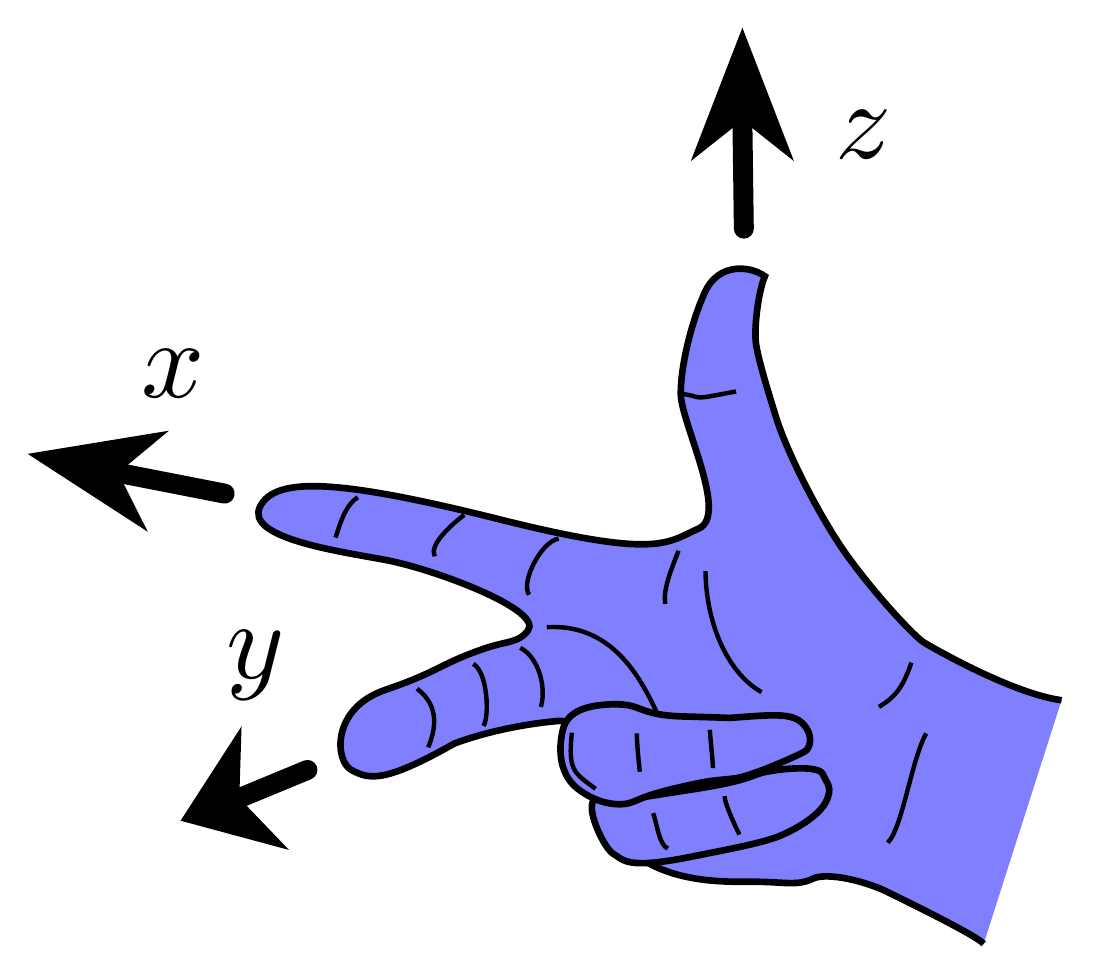
\begin{tikzpicture}[y=0.80pt, x=0.80pt, yscale=-1.000000, xscale=1.000000, inner sep=0pt, outer sep=0pt]
    \path[draw=black,fill=blue!50!white,line width=2.400pt] (466.9820,303.7880) ..
    controls (444.9820,300.7880) and (409.9820,280.7880) .. (404.9820,277.7880) ..
    controls (399.9820,274.7880) and (376.9820,249.7880) .. (364.9820,230.7880) ..
    controls (352.9820,211.7880) and (341.9820,188.7880) .. (337.9820,175.7880) ..
    controls (333.9820,162.7880) and (329.9820,149.7880) .. (328.9820,142.7880) ..
    controls (327.9820,135.7880) and (329.9820,119.2880) .. (332.9820,112.2880) ..
    controls (325.9820,107.2880) and (311.9820,106.2880) .. (305.9820,119.2880) ..
    controls (299.9820,132.2880) and (294.9820,152.2880) .. (294.9820,165.2880) ..
    controls (294.9820,178.2880) and (316.9820,220.2880) .. (302.9820,226.2880) ..
    controls (288.9820,232.2880) and (285.9820,240.2880) .. (213.9820,222.2880) ..
    controls (141.9820,204.2880) and (111.9820,202.2880) .. (104.9820,216.2880) ..
    controls (97.9820,230.2880) and (138.9820,236.2880) .. (160.9820,240.2880) ..
    controls (182.9820,244.2880) and (233.0030,262.9220) .. (225.9820,272.2880) ..
    controls (221.6320,278.0900) and (216.6070,276.7760) .. (205.2730,280.7760) ..
    controls (185.6620,287.6980) and (185.9650,290.7420) .. (161.4820,299.1210) ..
    controls (137.0490,307.4830) and (138.6390,331.3470) .. (146.3150,335.3510) ..
    controls (153.9910,339.3550) and (160.3310,341.6930) .. (192.7010,323.3380) ..
    controls (207.0510,317.9980) and (224.4830,314.4530) .. (239.8160,313.1200) ..
    controls (255.1490,311.7870) and (264.4840,369.1200) .. (281.1500,377.7870) ..
    controls (297.8160,386.4540) and (317.1490,385.7870) .. (329.1490,385.7870) ..
    controls (341.1490,385.7870) and (347.8150,387.7880) .. (354.4820,384.4540) ..
    controls (361.1490,381.1200) and (379.8160,385.7860) .. (389.8160,391.1200) ..
    controls (389.8160,391.1200) and (428.4830,409.7870) .. (431.8160,413.7870);
    \path[draw=black,line width=1.600pt] (234.4830,270.7870) .. controls
    (268.4820,268.7880) and (280.4820,301.4540) .. (288.4820,318.7880);
    \path[draw=black,line width=1.600pt] (306.1490,245.4530) .. controls
    (306.4830,270.7870) and (317.1500,292.1210) .. (331.4820,300.1190);
    \path[draw=black,line width=1.600pt] (239.8160,230.7870) .. controls
    (231.8160,232.1200) and (222.4830,250.7870) .. (226.4830,256.1200);
    \path[draw=black,line width=1.600pt] (197.1490,220.1200) .. controls
    (191.8160,224.1200) and (181.1490,233.4530) .. (183.8160,238.7870);
    \path[draw=black,line width=1.600pt] (149.1490,212.1200) .. controls
    (142.4820,216.1200) and (140.3150,227.6210) .. (138.9820,230.2870);
    \path[draw=black,line width=1.600pt] (222.4830,280.1210) .. controls
    (230.4830,284.1210) and (234.4830,297.4530) .. (231.8160,306.7870);
    \path[draw=black,line width=1.600pt] (201.2960,287.3930) .. controls
    (207.9630,291.3930) and (208.5440,311.3860) .. (205.8770,315.3860);
    \path[draw=black,line width=1.600pt] (175.8480,298.5900) .. controls
    (184.4960,305.0750) and (185.4390,314.1240) .. (180.9370,325.0560);
    \path[draw=black,line width=1.600pt] (293.9820,236.2880) .. controls
    (289.9820,246.2880) and (286.9820,254.2880) .. (287.9820,260.2880);
    \path[draw=black,line width=1.600pt] (294.9820,165.2880) .. controls
    (306.9290,166.9950) and (297.6590,168.5400) .. (319.9820,164.2880);
    \path[draw=black,line width=1.600pt] (399.1490,286.7880) .. controls
    (395.1490,298.7880) and (391.1490,302.7870) .. (384.4820,306.7870);
    \path[draw=black,fill=blue!50!white,line width=2.400pt] (299.8160,374.4550) ..
    controls (315.7210,371.2740) and (327.1500,369.1220) .. (335.8160,366.4550) ..
    controls (344.4820,363.7880) and (357.1480,356.4540) .. (360.4820,349.7880) ..
    controls (363.8160,343.1220) and (361.1490,341.7890) .. (359.1490,337.1220) ..
    controls (357.1490,332.4550) and (335.1500,335.1220) .. (329.8160,337.1220) ..
    controls (324.4820,339.1220) and (319.8160,341.1220) .. (297.8160,344.4550) ..
    controls (275.8160,347.7880) and (269.8160,349.4550) .. (258.4820,348.1210) ..
    controls (249.1900,347.0270) and (259.8170,370.4540) .. (264.4830,373.1210) ..
    controls (269.1490,375.7880) and (269.8160,380.4550) .. (299.8160,374.4550) --
    cycle;
    \path[draw=black,fill=blue!50!white,line width=2.400pt] (316.7840,311.7880) ..
    controls (335.6810,310.4550) and (345.1320,309.1220) .. (350.2190,314.4550) ..
    controls (355.3060,319.7880) and (353.1250,325.1220) .. (351.6720,326.4550) ..
    controls (350.2190,327.7880) and (333.5010,335.1210) .. (324.7790,337.7880) ..
    controls (316.0560,340.4550) and (314.6030,338.4550) .. (297.1600,342.4550) ..
    controls (279.7160,346.4550) and (278.2630,347.7880) .. (273.1740,349.7880) ..
    controls (268.0860,351.7880) and (257.9110,351.1210) .. (248.4630,343.7880) ..
    controls (239.0140,336.4550) and (240.4670,323.7880) .. (241.1940,319.7880) ..
    controls (241.9210,315.7880) and (242.6490,307.1210) .. (260.8190,305.7880) ..
    controls (278.9890,304.4550) and (273.1730,310.4540) .. (296.4330,311.1210) ..
    controls (319.6910,311.7880) and (316.7840,311.7880) .. (316.7840,311.7880) --
    cycle;
    \path[draw=black,line width=1.600pt] (245.8150,318.4550) .. controls
    (243.8920,335.7600) and (246.9240,336.6210) .. (256.4820,343.7880);
    \path[draw=black,line width=1.600pt] (275.1490,318.7870) .. controls
    (275.1490,324.1200) and (276.4820,336.1200) .. (276.4820,336.1200);
    \path[draw=black,line width=1.600pt] (308.1490,317.1200) .. controls
    (308.1490,319.7870) and (309.4830,330.4530) .. (309.4830,334.4530);
    \path[draw=black,line width=1.600pt] (314.8150,347.1220) .. controls
    (314.8150,351.1220) and (321.4820,364.4550) .. (321.4820,364.4550);
    \path[draw=black,line width=1.600pt] (282.4820,354.7880) .. controls
    (283.8150,357.4550) and (285.1490,369.4540) .. (289.1490,370.7880);
    \path[draw=black,line width=1.600pt] (405.8150,318.7880) .. controls
    (399.1490,330.7880) and (395.1490,361.4560) .. (388.4820,368.1220);
    \path[draw=black,fill=black,line cap=round,line width=7.200pt]
    (323.4820,90.7880) -- (322.8140,41.7880);
    \path[fill=black] (322.8140,41.7880) -- (299.5010,60.3000) -- (322.8140,0.0000)
    -- (346.1270,60.3000) -- cycle;
    \path[draw=black,fill=black,line cap=round,line width=7.200pt]
    (88.9960,210.4600) -- (40.9000,201.0670);
    \path[fill=black] (40.9000,201.0670) -- (54.2400,227.6800) -- (0.0000,192.5000)
    -- (63.7990,182.0440) -- cycle;
    \path[draw=black,fill=black,line cap=round,line width=7.200pt]
    (126.3770,335.2550) -- (95.5850,348.0050);
    \path[fill=black] (95.5850,348.0050) -- (118.0640,371.4130) --
    (69.0630,358.1970) -- (96.6050,315.5680) -- cycle;
    \path[fill=black,line join=miter,line cap=butt,line width=0.800pt]
    (51.2201,166.8365) node[above right] (text4204) {\scalebox{4}{$x$}};
    \path[fill=black,line join=miter,line cap=butt,line width=0.800pt]
    (89.7117,303.4817) node[above right] (text4208) {\scalebox{4}{$y$}};
    \path[fill=black,line join=miter,line cap=butt,line width=0.800pt]
    (364.9268,59.0600) node[above right] (text4212) {\scalebox{4}{$z$}};
  \end{tikzpicture}
\end{image}
Of course you will need to ``spin'' your hand around to align your
pointer-finger with the $x$-axis and your middle-finger with the
$y$-axis.
\begin{question}
  Which of the following axes are aligned according to the right-hand rule?
  \begin{hint}
    Point your pointer finger of your right hand in the positive
    direction of $x$-axis while simultaneously pointing your middle
    finger in the positive direction of $y$-axis. Your thumb will point
    in the positive direction of the $z$-axis.
  \end{hint}
   \begin{selectAll}
     \choice[correct]{
       \begin{tikzpicture}[baseline=2ex]
         \draw[->] (0,0)--(1,0);
         \draw[->] (0,0)--(0,1);
         \draw[->] (0,0)--(-.4,-.7);
         \node[right] at (1,0) {$y$};
         \node[above] at (0,1) {$z$};
         \node[below] at (-.4,-.7) {$x$};
     \end{tikzpicture}}
     \choice{
       \begin{tikzpicture}[baseline=2ex]
         \draw[->] (0,0)--(1,0);
         \draw[->] (0,0)--(0,1);
         \draw[->] (0,0)--(-.4,-.7);
         \node[right] at (1,0) {$y$};
         \node[above] at (0,1) {$x$};
         \node[below] at (-.4,-.7) {$z$};
     \end{tikzpicture}}
     \choice{
       \begin{tikzpicture}[baseline=2ex]
         \draw[->] (0,0)--(1,0);
         \draw[->] (0,0)--(0,1);
         \draw[->] (0,0)--(-.4,-.7);
         \node[right] at (1,0) {$x$};
         \node[above] at (0,1) {$z$};
         \node[below] at (-.4,-.7) {$y$};
     \end{tikzpicture}}
     \choice[correct]{
       \begin{tikzpicture}[baseline=2ex]
         \draw[->] (0,0)--(1,0);
         \draw[->] (0,0)--(0,1);
         \draw[->] (0,0)--(-.4,-.7);
         \node[right] at (1,0) {$z$};
         \node[above] at (0,1) {$x$};
         \node[below] at (-.4,-.7) {$y$};
     \end{tikzpicture}}
   \end{selectAll}
\end{question}




\section{Basic planes}

We can clearly see the $(x,y)$-plane in our axes
\begin{image}[2in]
  \begin{tikzpicture}
    \draw[draw=none,fill=fill1] (1.2,-.3)--(1.2,.9)--(-1,.9)--(-1,-.3)--(1.2,-.3);
    \draw[->] (0,0)--(1,0);
    \draw[->] (0,0)--(0,1);
    \draw[->] (0,0)--(-.4,-.7);
    \node[right] at (1,0) {$x$};
    \node[above] at (0,1) {$y$};
    \node[below] at (-.4,-.7) {$z$};
  \end{tikzpicture}
\end{image}
but there are also two other planes containing the lines of our axes:
$(x,z)$-plane, and the $(y,z)$-plane.

\begin{question}
  The $(y,z)$-plane corresponds to which of the following
  equations?
  \begin{multipleChoice}
    \choice[correct]{$x=0$}
    \choice{$y=0$}
    \choice{$z=0$}
  \end{multipleChoice}
  \begin{hint}
    Every point on the $(y,z)$-axis has $x=0$, so this is the answer.
  \end{hint}
\end{question}

\begin{question}
  Which of the following most accurately describes the solution
  set of $y=2$ in $\R^3$?
  \begin{multipleChoice}
    \choice{a horizontal line}
    \choice{a vertical line}
    \choice{a plane parallel to the $(x,y)$-plane}
    \choice[correct]{a plane parallel to the $(x,z)$-plane}
    \choice{a plane parallel to the $(y,z)$-plane}
  \end{multipleChoice}
  \begin{hint}
    $y=2$ consists of all those points where $y=2$, but $x$ and
    $z$ are allowed to be anything.  
  \end{hint}
\end{question}

%% Lines and planes
%% Ax+ by=c standard form ANY line.
%% In 3 D?

\section{Distance and spheres}

Suppose you want to know the distance between two points $(x,y)$ and
$(a,b)$. To do this, we use the distance formula!
\begin{theorem}
  Given two points $(x,y)$ and $(a,b)$ in $\R^2$, the distance between
  them is given by:
  \[
  \sqrt{(x-a)^2 + (y-b)^2}
  \]
  \begin{explanation}
    This is nothing more than a corollary of the Pythagorean
    Theorem. Plot the points $(a,b)$ and $(x,y)$:
    \begin{image}
      \begin{tikzpicture}
	\begin{axis}[
            xmin=0, xmax=5,ymin=0,ymax=5,
            axis lines =left, 
            every axis y label/.style={at=(current axis.above origin),anchor=south},
            every axis x label/.style={at=(current axis.right of origin),anchor=west},
            xtick={1,3}, xticklabels={$a$,$x$},
            ytick={2,3}, yticklabels={$b$,$y$},
            axis on top,
          ]       
          \addplot[penColor,dashed] plot coordinates {(1,0) (1,2)};
          \addplot[penColor,dashed] plot coordinates {(0,2) (1,2)};
          \addplot[penColor,dashed] plot coordinates {(3,0) (3,3)};
          \addplot[penColor,dashed] plot coordinates {(0,3) (3,3)};
          \addplot[penColor,only marks,mark=*] coordinates{(1,2)};  %% closed hole          
          \addplot[penColor,only marks,mark=*] coordinates{(3,3)};  %% closed hole          
        \end{axis}
      \end{tikzpicture}
    \end{image}
    We may now construct a right triangle with horizonatal side length
    $\answer[given]{(x-a)}$ and vertical side length
    $\answer[given]{(y-b)}$ whose hypotenuse is the shortest path
    between the two points:
    \begin{image}
      \begin{tikzpicture}
        \begin{axis}[
            xmin=0, xmax=5,ymin=0,ymax=5,
            axis lines =left, 
            every axis y label/.style={at=(current axis.above origin),anchor=south},
            every axis x label/.style={at=(current axis.right of origin),anchor=west},
            xtick={1,3}, xticklabels={$a$,$x$},
            ytick={2,3}, yticklabels={$b$,$y$},
            axis on top,
          ]       
          \node at (axis cs:2,1.75) {$(x-a)$}; 
          \node at (axis cs:3.5,2.5) {$(y-b)$}; 
          \addplot[dashed] plot coordinates {(1,2) (3,3)};
          \addplot[penColor] plot coordinates {(1,2) (3,2)};
          \addplot[penColor] plot coordinates {(3,2) (3,3)};
          \addplot[penColor] plot coordinates {(2.83,2) (2.83,2.2) (3,2.2)};
          \addplot[penColor,only marks,mark=*] coordinates{(1,2)};  %% closed hole          
          \addplot[penColor,only marks,mark=*] coordinates{(3,3)};  %% closed hole          
        \end{axis}
      \end{tikzpicture}
    \end{image}
    By the Pythagorean theorem, the length of this path is given by 
    \[
    \sqrt{(x-a)^{2}+(y-b)^{2}}.
    \]
  \end{explanation}
\end{theorem}

\begin{question}
  What is the distance between the points $(-17,379)$ and $(14,-101)$?
  \begin{prompt}
    The distance is $\answer{481}$ units.
  \end{prompt}
\end{question}

The distance formula also extends to higher dimensions:


\begin{theorem}
  Given two points $(x,y,z)$ and $(a,b,c)$ in $\R^3$, the distance between
  them is given by:
  \[
  \sqrt{(x-a)^2 + (y-b)^2 + (z-c)^2}
  \]
  \begin{explanation}
  \end{explanation}
\end{theorem}

\begin{question}
\end{question}




\subsection{Circles and spheres, disks and balls}

Just as the equation of a circle is related to the distance formula in
$\R^2$, the equation of a sphere is related to the distance formula in
$\R^3$:


\begin{theorem}
  The equation for a circle of radius $r$ centered at the point
  $(a,b)$ in $\R^2$ is
  \[
  r^2=(x-a)^2 + (y-b)^2
  \]
  The equation for a sphere of radius $r$ centered at the point
  $(a,b,c)$ in $\R^3$ is
  \[
  r^2 = (x-a)^2 + (y-b)^2 + (x-c)^2
  \]
  In general, the equation for a $n$-dimensional ``sphere'' of radius
  $r$ centered at the point $(a_1,a_2,a_3,\dots,a_n)$ is
  \[
  r^2 = \sum_{i=1}^n(x-a_i)^2
  \]
  \begin{explanation}
    This follows directly from the distance formula since a sphere is
    the set of points that are equidistant from a given point.
  \end{explanation}
\end{theorem}

\begin{corollary}
  In general, the equation for a $n$-dimensional ``ball'' of radius
  $r$ centered at the point $(a_1,a_2,a_3,\dots,a_n)$ is
  \[
  r^2 \ge \sum_{i=1}^n(x-a_i)^2
  \]
  \begin{explanation}
    Here the ``$\ge$'' fills-in the $n$-dimensional sphere.
  \end{explanation}
\end{corollary}


\begin{question}
  The equation $(x-1)^2+y^2+(z+2)^2 = 4$ has a solution set in
  $\R^3$ which is a sphere.  What is the center and
  radius of this sphere?
  \begin{prompt}
  \[
  \text{Radius} = \answer{2}
  \]
  \[
  \text{Center} = \left(\answer{1},\answer{0}, \answer{-2} \right)
  \]
  \end{prompt}
  \begin{hint}
    $(x-1)^2+y^2+(z+2)^2$ is the square of the distance from
    $(1,0,-2)$ to $(x,y,z)$.  If the square of the distance is $4$, then
    the distance is $2$.  Since the solution set of this equation is all
    points which are a distance of $2$ away from $(1,0,-2)$, then this
    is a sphere of radius $2$ centered at $(1,0,-2)$
  \end{hint}
\end{question}


\section{Notation for functions}

In this course we will be working with functions that could have multiple
inputs and multiple outputs. We will try to adhere to the following
(nonstandard!) convention to aid the young mathematician:

\begin{itemize}
  \item The \textbf{case} of the function will denote the number of
    \textbf{inputs}, with lowercase indicating a single input, and uppercase
    indicating multiple inputs.
  \item The \textbf{face} of the function will denote the number of
    \textbf{outputs}, with normalface ($f$ or $F$) indicating a single
    output, and boldface ($\vec{f}$, and $\vec{F}$) indicating multiple
    outputs.
\end{itemize}
Hence we could have functions that map:
\begin{itemize}
\item $f:\R \to \R$
\item $\vec{f}:\R \to \R^2$
\item $\vec{f}:\R \to \R^3$
\item $F:\R^2\to \R$
\item $F:\R^3\to \R$
\item $\vec{F}:\R^2 \to \R^2$
\item $\vec{F}:\R^3 \to \R^3$
\end{itemize}
\end{document}
